\chapter{Tagsets with Streams}
\index{Streams}
Streams add another level of versatility to tagsets.  
Streams allow for output to be saved away, and reused or
just delayed.  This is ideal for solving problems where
the ODS event model does not match the shape of the target
ouput. Streams are the most common solution to this problem.
Streams can delay output, collect output from different events
at different times, to be used later.
This chapter will show how to use streams to solve problems
that would otherwise be impossible.

\section{A Tagset with Startpage}
\index{Tagsets!StartPage}
\index{StartPage}
\index{Titles}
\index{Footnotes}
\index{Page breaks}
Several of the ODS destinations have an option called startpage.
Startpage has at least two options, on and off.  On is normal behavior.
Off means that pagebreaks, titles and footnotes are suppressed.  There
are several other possible values for startpage,  the only one that 
makes much sense for a tagset is 'now'.  Now means that the footnotes,
pagebreak and titles should happen next.

ODS markup does not have a startpage option yet.  But startpage behavior
can be implemented with a tagset.  This tagset will use streams to catch the
titles and footnotes.  The emphasis of this tagset is on entirely new
events that have been mostly ignored until now.

\subsection{Identify, Locate and Explore}
Running the code below will give us a nice event map with easy
to find titles and footnotes.

\begin{verbatim}
Title '!!!!!!!!! My New Title !!!!!!!!!';
Footnote '######## My New Footnote ########';
ods tagsets.short_map file='map.xml';
proc print data=sashelp.class; run;
ods tagsets.short_map close;
\end{verbatim}

\index{Events!System\_Title\_setup\_group}
\index{Events!Title\_setup\_container}
\index{Events!System\_Title\_setup}
\index{Events!System\_Footer\_setup\_group}
\index{Events!Footer\_setup\_container}
\index{Events!System\_Footer\_setup}
\index{Events!page\_setup}
What you will find is that the titles and footnotes are listed twice.
Once in a page setup section, and once for each page.  Part of the
resulting output is shown on page \pageref{startpage_out}.
% in \ref{startpage_out} on page \pageref{startpage_out}.

\clearpage
\begin{fvoutput}{startpage_out}{Title and Footnote Events}
      <page_setup>
        <system_title_setup_group>
          <title_setup_container>
            <title_setup_container_specs>
              <title_setup_container_spec/>
            </title_setup_container_specs>
            <title_setup_container_row>
              <system_title_setup value="!!!!!!!!! My New Title !!!!!!!!!">
              </system_title_setup>
            </title_setup_container_row>
          </title_setup_container>
        </system_title_setup_group>
        <system_footer_setup_group>
          <title_setup_container>
            <title_setup_container_specs>
              <title_setup_container_spec/>
            </title_setup_container_specs>
            <title_setup_container_row>
              <system_footer_setup value="######## My New Footnote ########">
              </system_footer_setup>
            </title_setup_container_row>
          </title_setup_container>
        </system_footer_setup_group>
      </page_setup>
      <system_title_group>
        <title_container>
          <title_container_specs>
            <title_container_spec/>
          </title_container_specs>
          <title_container_row>
            <system_title value="!!!!!!!!! My New Title !!!!!!!!!">
            </system_title>
          </title_container_row>
        </title_container>
      </system_title_group>
...
...
...

      <system_footer_group>
        <title_container>
          <title_container_specs>
            <title_container_spec/>
          </title_container_specs>
          <title_container_row>
            <system_footer value="######## My New Footnote ########">
            </system_footer>
          </title_container_row>
        </title_container>
      </system_footer_group>

\end{fvoutput}

\index{Events!System\_Title\_setup\_group}
\index{Events!Title\_setup\_container}
\index{Events!System\_Title\_setup}
\index{Events!System\_Footer\_setup\_group}
\index{Events!Footer\_setup\_container}
\index{Events!System\_Footer\_setup}
The most useful thing about this output is that each set of titles
and footnotes is contained within group events.  There are System\_title\_group
and System\_footer\_group events as well as setup\_group events for each.  the
titles and footnotes can be captured by using those events to advantage.

\subsection{Defining the solution}
Inside the group events, there are title\_container events.  These events
are the same for both the titles and the footnotes.  The behavior of startpage, is
that titles, footnotes and pagebreaks are suppressed.  When it is turned on, titles
and footnotes come out as normal.  But while startpage was off, any footnotes that 
may have occured need to be saved and printed when the output ends, or startpage is
turned back on.   That's where the stream comes in.  It can be used to save the footnotes.

\subsection{Block and Unblock statments}
\index{Statements!Block}
\index{Statements!UnBlock}
\index{Block}
\index{UnBlock}
There are two more statements that will come in handy for this tagset.  The Block and unblock
statements will allow an event to be turned off and on.  One complication is that block and
unblock do reference counting.  In other words, if an event is blocked twice, it will have
to be unblocked twice before it will work again.  This behavior can be defeated by 
compartmentalizing the blocking behavior in an event or two.

\subsection{A partial solution}
\index{Events!pagebreak}
\index{Events!System\_Title}
\index{Events!System\_Footer}
\index{Events!Title\_container\_row}
\index{Events!Title\_container\_spec}
\index{Events!Title\_container\_specs}
A good place to start is to define events to block the titles, footnotes, and pagebreaks.  
By looking at the prevous map it is obvious  the title\_container, title\_container\_row,
system\_footer and system\_title events will need to be blocked.  There may be others
but it depends on what the html tagsets have defined.
This is a good start, if more events need blocking then they can be added later. There 
is no real need to turn anything on or off yet.  This is just a sanity check to see if
this will work as planned.

\index{Events!pagebreak}
\index{Events!Title\_container}
\index{Events!Title\_container\_row}
\index{Statements!Block}
\index{Statements!UnBlock}
\index{Block}
\index{UnBlock}
This example uses a separate event to block the different parts of
the output.  One event to block and unblock the title\_container
events, One each for the system\_title, system\_footer, and pagebreak
events. Each one keeps track of the blocking with a variable.  The
variable either exists with a value of 'True', or it doesn't.  This
keeps the tests simple and effecient. The start section is used to
do the blocking and the finish to do the unblocking. This nicely
compartmentalizes the block and unblock controls.

\begin{fvcode}{startpage1.sas}{Blocking the titles and footnotes}
proc template;
     define tagset tagsets.startpage;
         parent=tagsets.html4;
        /*-------------------------------------------------------eric-*/
        /*-- All titles happen between this event's start           --*/
        /*-- and finish.  redirect them to a stream or              --*/
        /*-- throw them away.                                       --*/
        /*----------------------------------------------------14Aug03-*/
        define event system_title_group;
            start:
                trigger block_title;
                trigger block_title_container;
                trigger block_page_breaks;
            finish:
                trigger block_title;
                trigger block_title_container;
        end;
        
        
        /*-------------------------------------------------------eric-*/
        /*-- All footnotes happen between this event's start        --*/
        /*-- and finish.  redirect them to a stream or              --*/
        /*-- throw them away.                                       --*/
        /*----------------------------------------------------14Aug03-*/
        define event system_footer_group;
            start:
                trigger block_footnote;
                trigger block_title_container;
            finish:
                trigger block_footnote finish;
                trigger block_title_container finish;
        end;
            
        /*--------------------------------------------------eric-*/
        /*-- Block/unblock the titles or footnotes.            --*/
        /*-----------------------------------------------11Aug03-*/
        define event block_title_container;
            start:
                break /if $title_container_blocked;
 
                unblock title_container;
                unblock title_row;
                set $title_container_blocked "true";
             finish:
                unblock title_container;
                unblock title_row;
                unset $title_container_blocked;
        end;
         

        define event block_title;
            start:
                break /if $title_blocked;
 
                block system_title;
                set $title_blocked "true";
            finish:
                unblock system_title;
                unset $title_blocked;
        end;

 
        define event block_footnote;
            start:
                break /if $footnote_blocked;

                block system_footer;
                set $footnote_blocked "true";
             finish:
                 unblock system_footer;
                 unset $footnote_blocked;
        end;
         

        /*-------------------------------------------------------eric-*/
        /*-- block the page breaks                                  --*/
        /*----------------------------------------------------1Aug 03-*/
        define event block_page_breaks;
            start:
                /*-----------------------------------------------eric-*/
                /*-- Only block it once.  Keep the reference count  --*/
                /*-- to one.                                        --*/
                /*--------------------------------------------14Aug03-*/
                do / if ^exists($page_blocked);
                    set $page_blocked "true";
                    block pagebreak;
                done;                   
            finish:
                unblock pagebreak;
                unset $page_blocked;
        end;
    end;
run;

Title '!!!!!!!!! My New Title !!!!!!!!!';
Footnote '######## My New Footnote ########';
ods tagsets.startpage file='startpage.html';
ods html file='startpage_compare.html';
proc print data=sashelp.class;run;
proc print data=sashelp.class;run;
ods _all_ close;

\end{fvcode}

\subsection{The Solution}
\index{Footnotes}
\index{Titles}
\index{page breaks}
Comparing the output from the startpage tagset with the html4 tagset shows that
the titles, footnotes and pagebreaks have been successfully removed.
The next step is to get the titles and footnotes back.  It's time to add a startpage option
to control when that will happen.

If startpage is set to 'no', titles should print once and then stop.  The first footnotes
encountered also need to be saved.  After some footnotes have been captured any footnotes
that follow can be thrown away.

If startpage is set to 'yes' everything is printed as normal.  For convenience, it is 
useful to create a put\_footnotes event that puts the footnote stream and deletes it.

\index{Footnotes}
Since only the first footnotes should print, the footnotes stream should only be opened if
if the stream is empty.  If the stream is not opened, it doesn't hurt anything to 
do a close.  It also doesn't hurt to unblock an event that is already unblocked.  Logic could
be added to avoid doing these unecessary things but the tagset becomes more complex without
any real benefit.
The output can be seen in figure \vref{startpage2_out}.


\begin{fvcode}{startpage2}{Startpage Tagset}
proc template;
    define tagset tagsets.startpage;
        parent=tagsets.html4;
        
        define event initialize;
            unset $start_page_no; 
            do /if $options;
                set $start_page_no "true" /if cmp($options['STARTPAGE']), 'no');
            done;
        end;    

        define event options_set;
            trigger initialize;
        end;

        /*-------------------------------------------------------eric-*/
        /*-- All titles happen between this event's start           --*/
        /*-- and finish.  redirect them to a stream or              --*/
        /*-- throw them away.                                       --*/
        /*----------------------------------------------------14Aug03-*/
        define event system_title_group;
            start:
                do /if $start_page_no;
                    do /if $titles_printed;
                        trigger block_title;
                        trigger block_title_container;
                    done;
                    set $titles_printed "true";

                    /*------------------------------------------eric-*/
                    /*-- Block the page breaks after the first     --*/
                    /*-- titles have been printed.  Otherwise we   --*/
                    /*-- don't get a pagebreak when we switch from --*/
                    /*-- start_page=yes to start_page=no.          --*/
                    /*---------------------------------------11Aug03-*/
                    trigger block_page_breaks start;
                done;
            finish:
                trigger block_title;
                trigger block_title_container;
        end;
        
        
        /*-------------------------------------------------------eric-*/
        /*-- All footnotes happen between this event's start        --*/
        /*-- and finish.  redirect them to a stream or              --*/
        /*-- throw them away.                                       --*/
        /*----------------------------------------------------14Aug03-*/
        define event system_footer_group;
            start:
                do /if exists($$footnotes);
                    trigger block_footnote;
                    trigger block_title_container;
                else;
                    open footnotes;
                done;

            finish:
                close;
                unset $footnotes_open;
                trigger block_footnote;
                trigger block_title_container;

                trigger put_footnotes /if ^$start_page_no;
        end;
            

        /*-------------------------------------------------------eric-*/
        /*-- Write out the footnotes we saved earlier.              --*/
        /*----------------------------------------------------14Aug03-*/
        define event put_footnotes;
            put $$footnotes;
            unset $$footnotes;
        end;
        
            
        /*--------------------------------------------------eric-*/
        /*-- Block/unblock the titles or footnotes.            --*/
        /*-----------------------------------------------11Aug03-*/
        define event block_title_container;
            start:
                break /if $title_container_blocked;
 
                unblock title_container;
                unblock title_row;
                set $title_container_blocked "true";
             finish:
                unblock title_container;
                unblock title_row;
                unset $title_container_blocked;
        end;
         

        define event block_title;
            start:
                break /if $title_blocked;
 
                block system_title;
                set $title_blocked "true";
            finish:
                unblock system_title;
                unset $title_blocked;
        end;

 
        define event block_footnote;
            start:
                break /if $footnote_blocked;

                block system_footer;
                set $footnote_blocked "true";
             finish:
                 unblock system_footer;
                 unset $footnote_blocked;
        end;
         

        /*-------------------------------------------------------eric-*/
        /*-- block the page breaks so we don't get them inside the panel.--*/
        /*----------------------------------------------------1Aug 03-*/
        define event block_page_breaks;
            start:
                /*-----------------------------------------------eric-*/
                /*-- Only block it once.  Keep the reference count  --*/
                /*-- to one.                                        --*/
                /*--------------------------------------------14Aug03-*/
                do / if ^exists($page_blocked);
                    set $page_blocked "true";
                    block line;
                    block pagebreak;
                done;                   
            finish:
                unblock line;
                unblock pagebreak;
                unset $page_blocked;
        end;

    end;
run;

Title '!!!!!!!!! My New Title !!!!!!!!!';
Footnote '######## My New Footnote ########';

options obs=1;

ods tagsets.startpage file='startpage.html' options(startpage='no');
proc print data=sashelp.class;run;
proc print data=sashelp.class;run;
ods _all_ close;

\end{fvcode}

\begin{goutput}{startpage1_out}{Start Page Working}
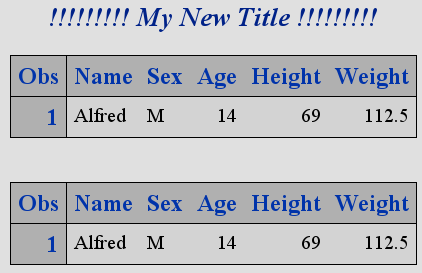
\includegraphics[width=6in]{startpage1.png}
\end{goutput}


\subsection{More Identify and Locate}
\index{Footnotes}
\index{Events!doc\_body}
So far so good, but where are the footnotes? They never get printed
because startpage is always no! Something needs to print them when
the document finishes, regardless of the setting of startpage.
Looking at the HTML from the first example it can be seen that the
footnotes came out right above the closing </body> tag.  Looking
through the html tagsets for the body tag gives away the the doc\_body
event.  The html4 tagset inherits the doc\_body event from the htmlcss
tagset.  All that is needed is to trigger the put\_footnotes event
in the finish of the doc\_body event.  There won't be any footnotes
to print if they've been printed already.

\begin{sfvcode}
proc template;
    define tagset tagsets.startpage2;
        parent=tagsets.startpage;
        
        define event doc_body;
            start:
                put '<body onload="startup()"';
                put ' onunload="shutdown()"';
                put  ' bgproperties="fixed"' / WATERMARK;
                putq " class=" HTMLCLASS;
                putq " background=" BACKGROUNDIMAGE;
                trigger style_inline;
                put ">" CR;
                trigger pre_post;
                put          CR;
                trigger ie_check;

            finish:
                trigger put_footnotes;

                trigger pre_post;
                put "</body>" CR;
        end;
    end;
run;

Title '!!!!!!!!! My New Title !!!!!!!!!';
Footnote '######## My New Footnote ########';

options obs=1;

ods tagsets.startpage2 file='startpage.html' options(startpage='no');
proc print data=sashelp.class;run;
proc print data=sashelp.class;run;
ods _all_ close;
\end{sfvcode}

\begin{goutput}{startpage2_out}{Start Page Working}
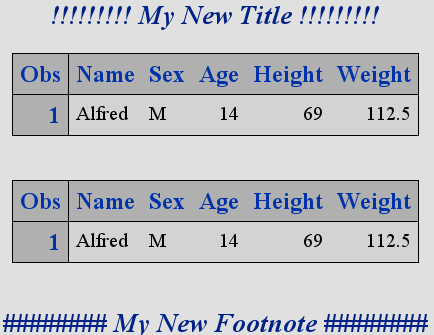
\includegraphics[width=6in]{startpage2.png}
\end{goutput}


\begin{sfvcode}
proc template;
/* start it off with startpage=no. */
ods tagsets.startpage2 options(startpage="no") file="startpage.html";

proc print data=sashelp.class; run;

proc print data=sashelp.class; run;

ods tagsets.startpage2 options(startpage="yes");

proc print data=sashelp.class; run;

proc print data=sashelp.class; run;

ods tagsets.startpage2 options(startpage="no");

proc print data=sashelp.class; run;

proc print data=sashelp.class; run;

ods _all_ close;
\end{sfvcode}

\begin{goutput}{startpage3_out}{Start Page }
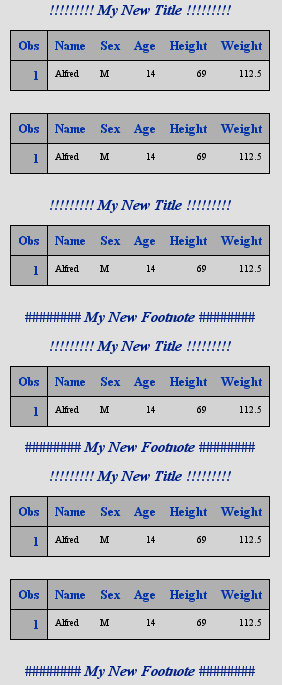
\includegraphics[width=3in]{startpage3.png}
\end{goutput}

\subsection{The Final Solution}
The output is shown in figure \vref{startpage3_out}.

\subsubsection{More exploration}
But there is something wrong.  The footnotes are missing from the first section. 
All the pagebreaks are missing.  Sprinkling a few putvars and putlog statements
through this tagset is helpful.

The startpage event is a boundry condition.  The footnotes need to be printed when
the value of start\_page changes to yes.  The pagebreaks are missing because they
get blocked once after the first titles are printed.  The startpage event needs
to unblock them in order for everything to return to normal.

Changing the startpage event to the following will fix everything.
The output is shown in figure \vref{startpage4_out}.

\begin{sfvcode}
        define event startpage;
            /*---------------------------------------------------eric-*/
            /*-- if we got a value check set start page,            --*/
            /*-- if we didn't get a value then set it               --*/
            /*-- to the alias we got on the initial ods             --*/
            /*-- statement.                                         --*/
            /*------------------------------------------------11Aug03-*/
            unset $start_page_no;

            do /if value;
                set $start_page_no 'true' /if cmp(value, 'no');
            else;
                set $start_page_no 'true' /if cmp(tagset_alias, 'no');
            done;
            
            do /if !$start_page_no;
                unset $start_page_no;
                unset $titles_printed;

                trigger put_footnotes;
                trigger block_page_breaks finish;
            done;
        end;
\end{sfvcode}

\begin{goutput}{startpage4_out}{Start Page - Final Version}
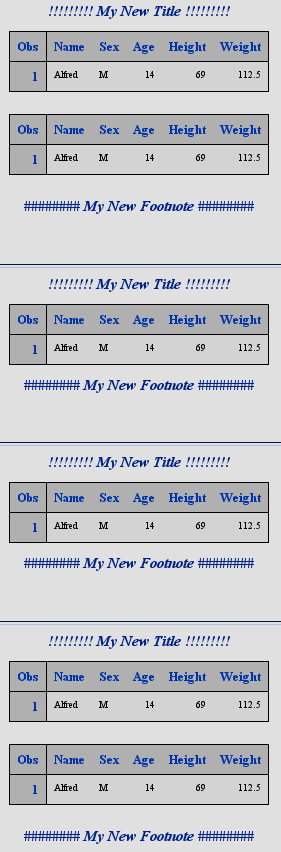
\includegraphics[width=3in]{startpage4.png}
\end{goutput}


\section{Summary}
Streams are one of the most powerful features available in tagsets.
They can be used to delay and repeat output or rearrange output to
fit your needs.  Streams do expose some difficulties presented by 
specific procedures but with careful consideration, thought and 
maybe a little frustration, those problems can be overcome.

